
La detección de muones en este proyecto es realizada mediante un detector de partículas inspirado en los detectores sTGC del proyecto ATLAS, en CERN. La sigla significa ''small Thin Gap Chamber", y forman parte de un espectrómetro de muones que permite conocer momento y trayectoria de estas partículas. Los muones proveen de información importante para la reconstrucción de eventos asociados a colisiones de partículas.

\begin{figure}[h]
	\centering
	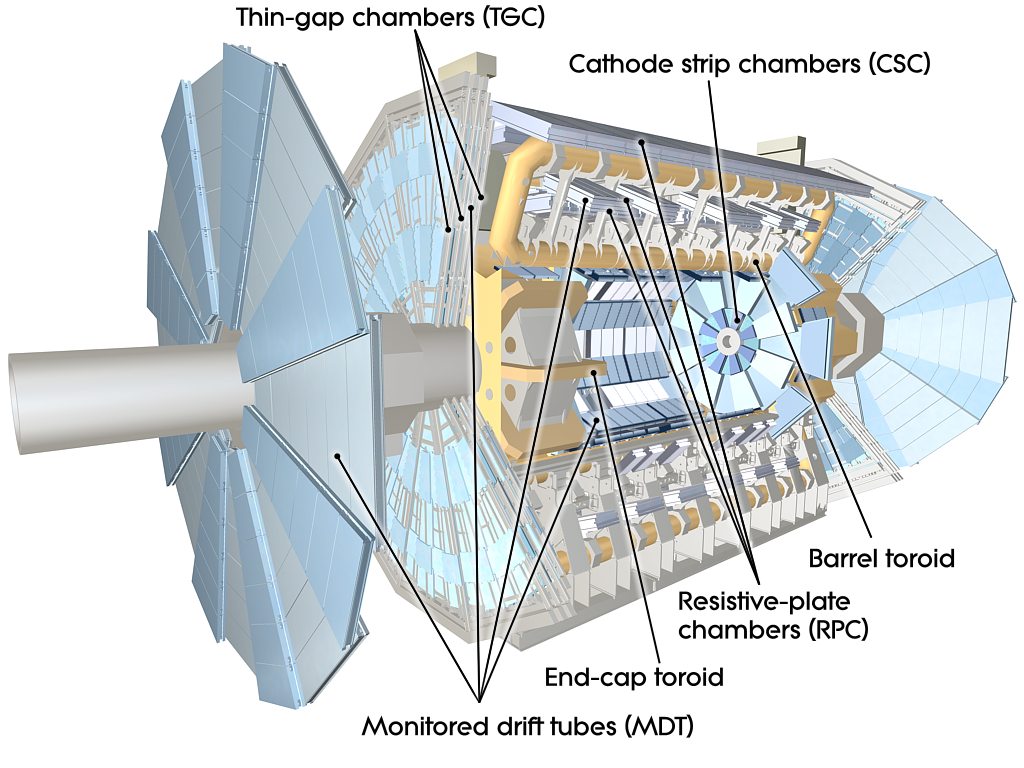
\includegraphics[scale=0.3]{atlas-muon-spectrometer-layout.png}
	\caption{Diagrama del espectrómetro de muones en el proyecto ATLAS\cite{AtlasMuonDiagram}.}
	\label{img:atlas-layout}
\end{figure}

\newpage
\begin{figure}[h]
	\centering
	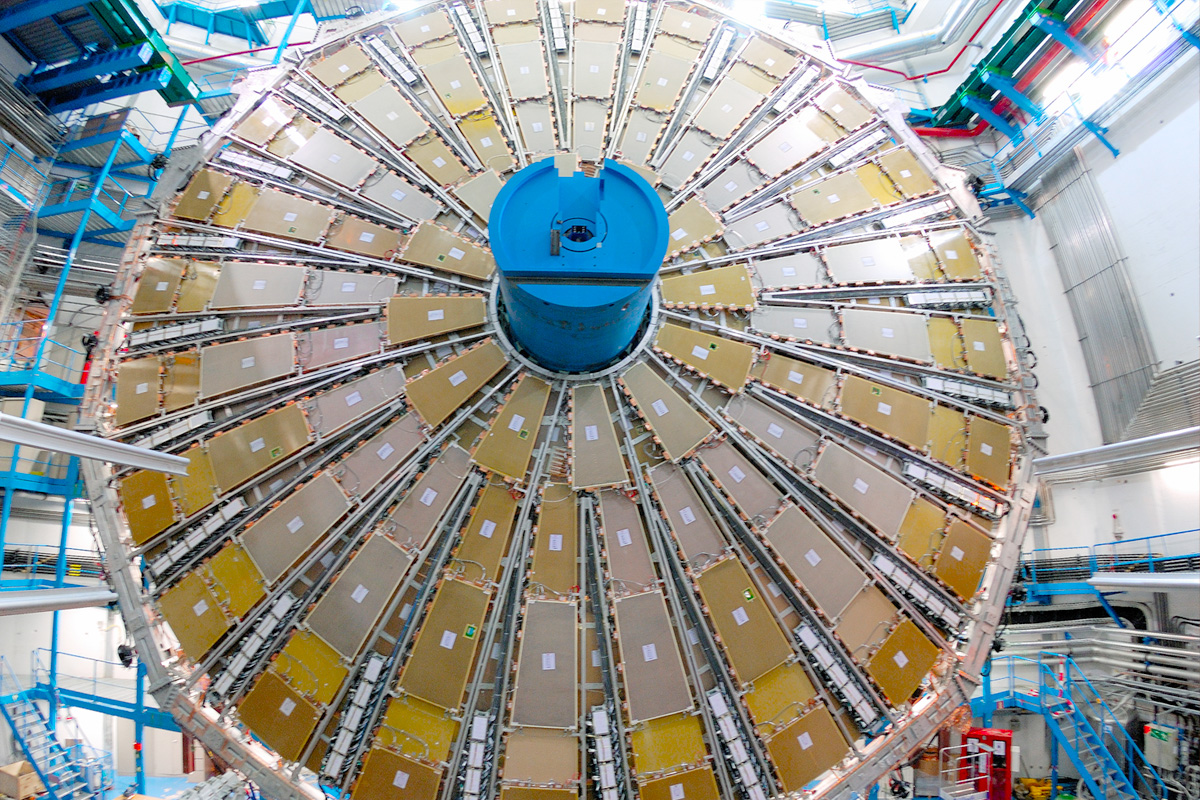
\includegraphics[scale=0.3]{atlas-muon-tgc.jpg}
	\caption{Fotografía del los detectores sTGC en el espectrómetro de muones del proyecto ATLAS\cite{AtlasMuonSpect}.}
	\label{img:atlas-tgc}
\end{figure}

\begin{figure}[h]
	\centering
	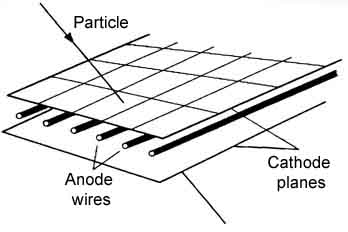
\includegraphics[scale=1]{stgc-lateral.jpg}
	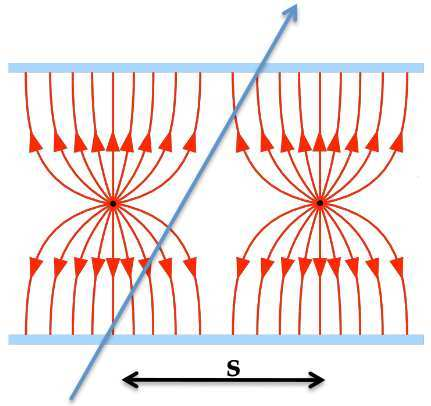
\includegraphics[scale=0.3]{stgc-transversal.png}
	\caption{Esquemas de un detector. La figura izquierda representa una vista lateral, mientras que la derecha ilustra un corte transversal del mismo. En ambos se observan  }
	\label{img:stgc-diagrams}
\end{figure}

\newpage
\subsection*{Estructura}

	Un TGC se compone de dos planos catódicos y varios cables anódicos. Los cátodos están seccionados en tiras llamadas "\textit{strips}". Los cables se encuentran ubicados perpendicularmente respecto a los \textit{strips}.
	
	Al interior del detector, entre los planos catódicos, se infiltra un gas compuesto por dióxido de carbono y pentano. Mediante la aplicación de alto voltaje, se genera un campo eléctrico entre ánodos y cátodos.
	
	El paso de muones a través del detector genera la ionización del gas y la liberación de electrones que son captados por los cables del detector. Este flujo de electrones genera pulsos de corriente tanto en los \textit{strips} como en los cables. Estos pulsos son de mayor amplitud en torno a la zona del evento ionizante, mientras que a mayor distancia la amplitud disminuye. Esto permite relacionar la posición y energía de la partícula con las amplitudes de los pulsos en cada \textit{strip} o cable.

\subsection*{Mini sTGC Utilizado}
	En ATLAS se leen tanto cátodos como ánodos. Esto permite trazar cuadrantes de posición del evento, ya que los \textit{strips} son perpendiculares a los cables. En este proyecto de titulación se leerán solo las señales provenientes de los \textit{strips} catódicos, por los que solo se mide un eje de posición. 
	
	Para agregar un eje adicional, se superpone un segundo TGC con \textit{strips} perpendiculares al detector anterior. Así se puede tener información bidimensional del paso de una partícula leyendo solo los cátodos. De este modo, el detector utilizado para este proyecto de titulación corresponde a dos mini-detectores TGC superpuestos, con \textit{strips} perpendiculares entre sí.
	
	\begin{figure}
		\centering
		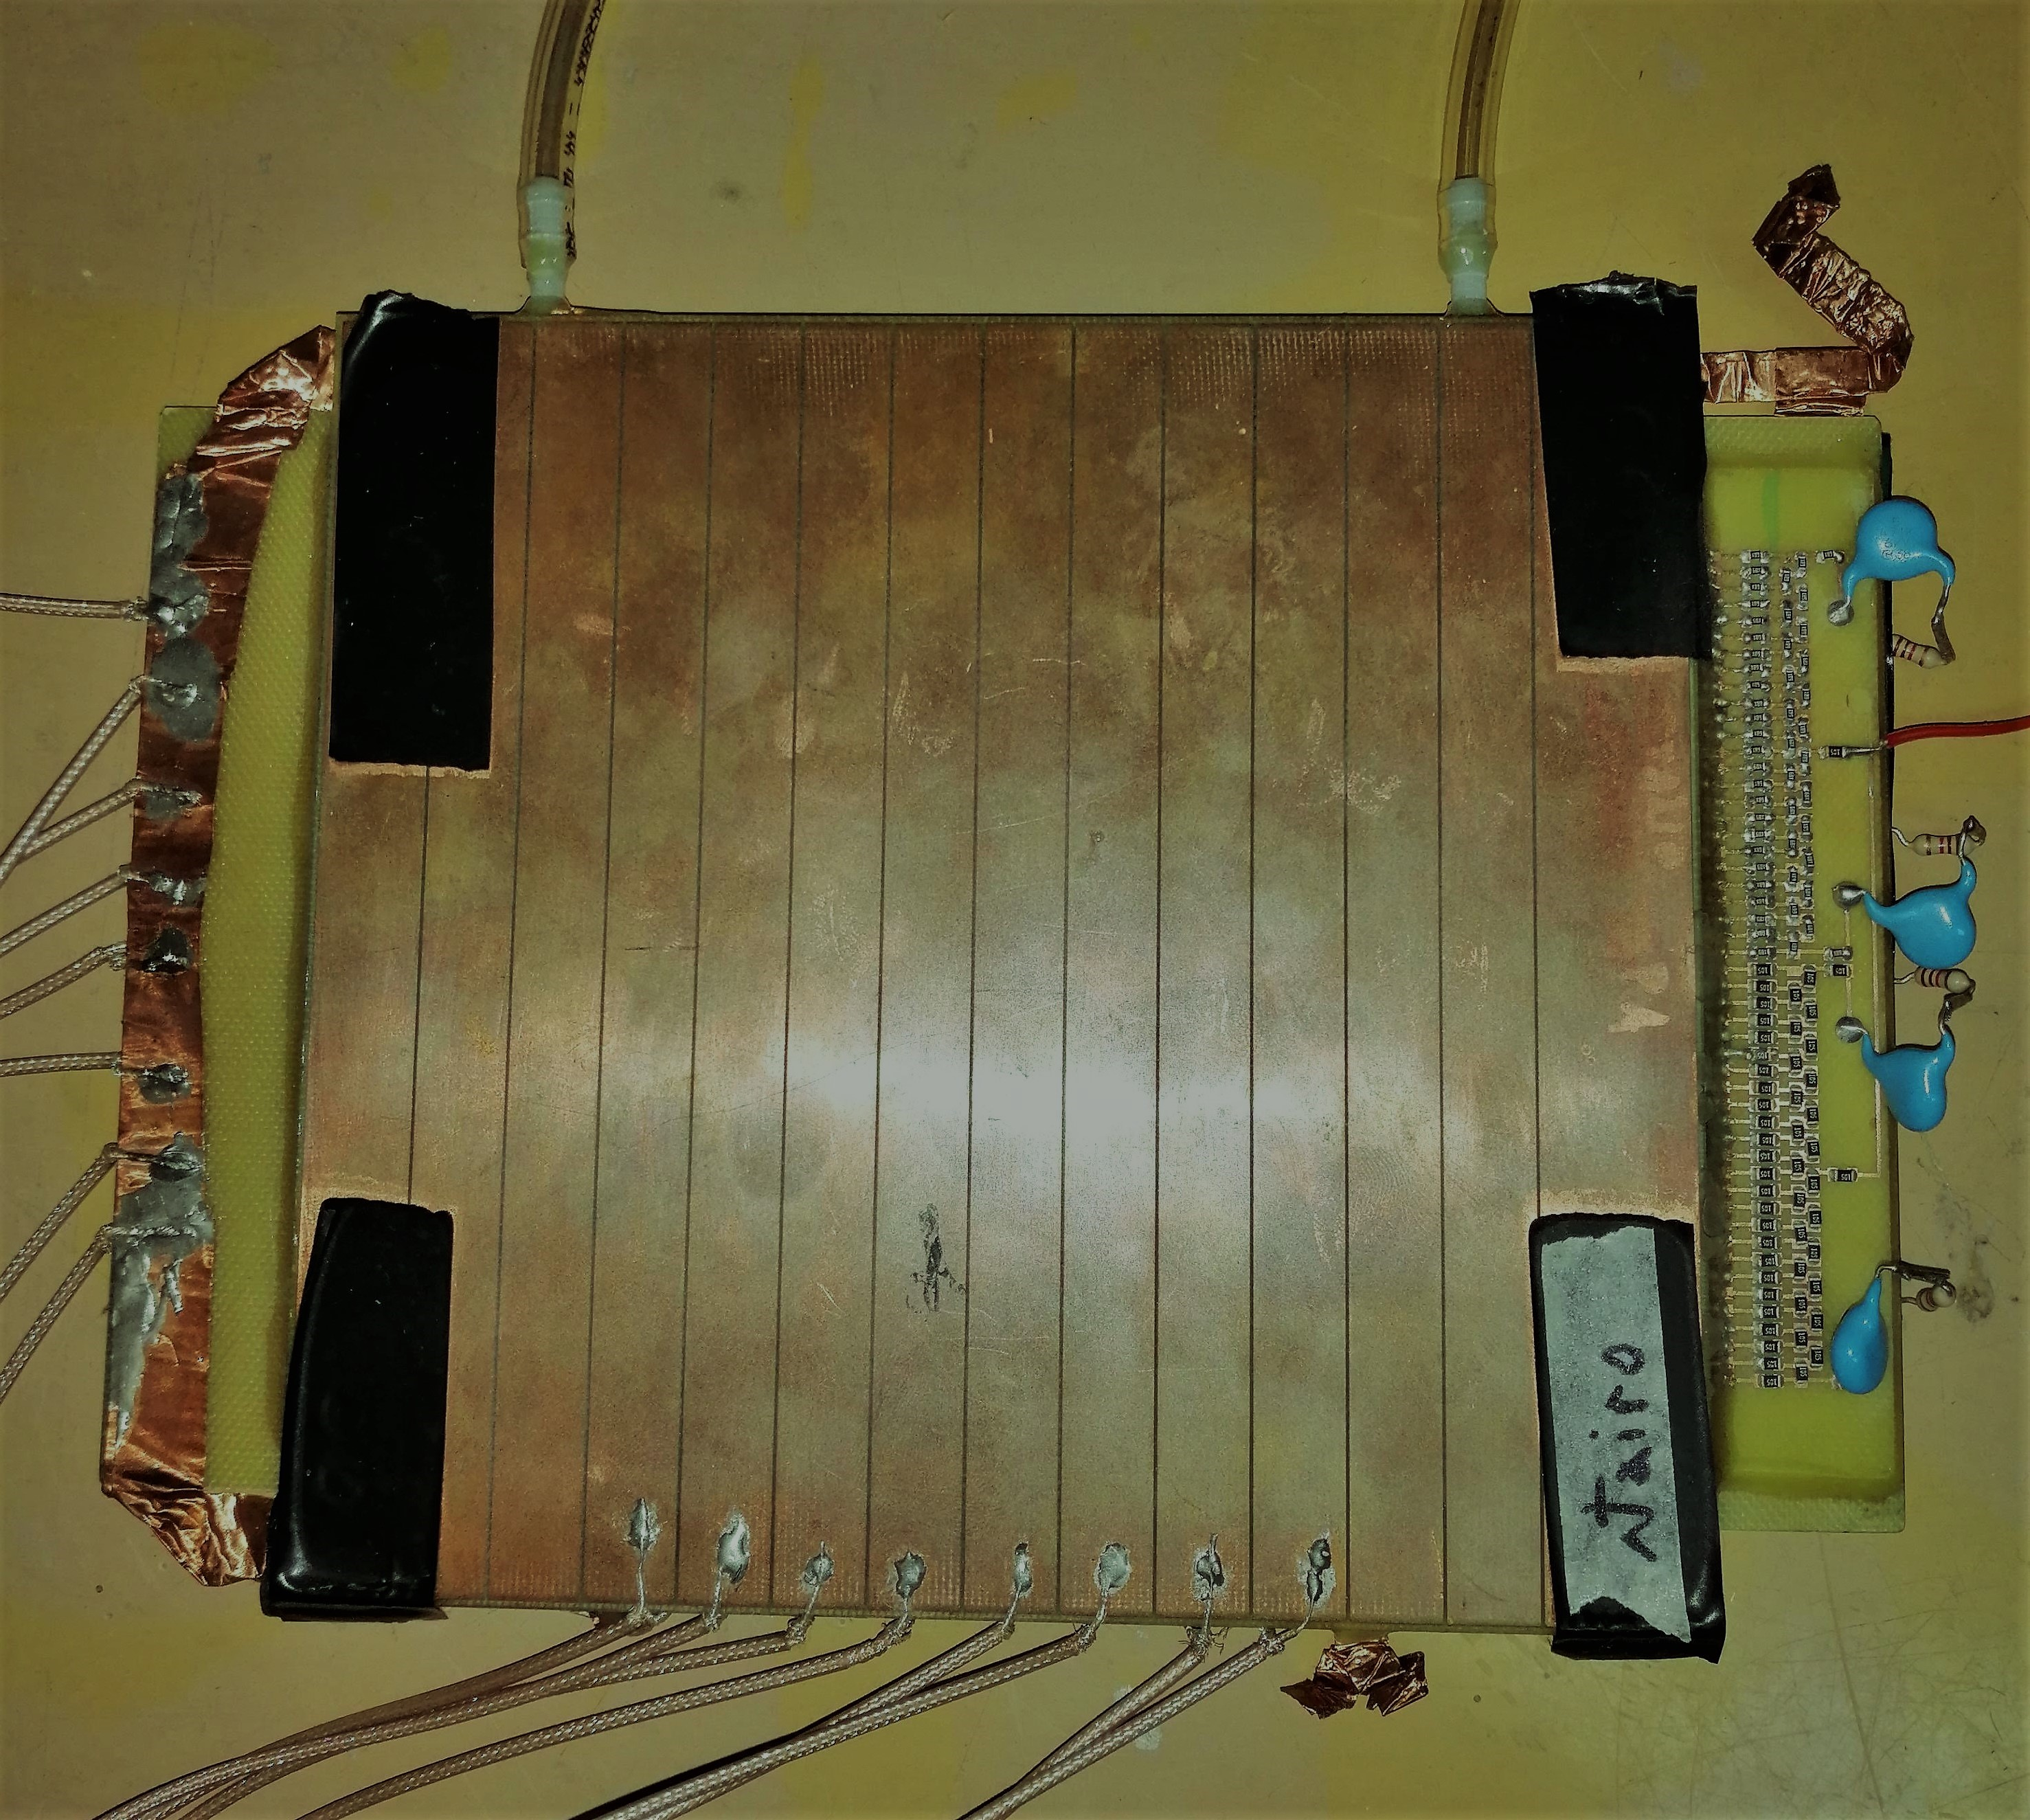
\includegraphics[scale=0.1]{mini-stgc.jpg}
		\caption{Vista superior del detector utilizado. Arriba se observan tubos para el flujo de gas. Abajo se ubican 8 cables coaxiales conectados a los \textit{strips} centrales de una cara del detector. A la izquierda están situados los otros 8 cables correspondientes a los \textit{strips} de la cara inferior. En el costado derecho se observa una red resistiva ponderadora para la lectura de los cables internos del detector, los cuales no serán utilizados en este proyecto.}
		\label{img:foto-mini-stgc}
	\end{figure}
	
	En particular, el detector utilizado cuenta con 8 \textit{strips} útiles, de 15 centímetros largo y 1 centímetro de ancho por cada sub-detector. El gas se ioniza con 3000VDC y una corriente límite de 50uA. El gas en su interior puede ser dióxido de carbono puro, con el compromiso de generar mayor cantidad de descargas no asociadas a muones.


%pruebas, gráficos, entradas y salidas, triggers, plásticos, fuentes radioactivas